\documentclass[12pt]{article}
\usepackage{amsmath}
\usepackage{jheppub}

\newcommand{\IGNORE}[1]{}
\newcommand{\be}{\begin{equation}}
\newcommand{\ee}{\end{equation}}

\title{Gibbons-Hawking-York Boundary Term in Causal Sets}
 \author[a]{M. Buck}
 \author[a,b]{\!, F. Dowker}
 \author[a]{and I. Jubb\,}
\affiliation[a]{Theoretical Physics Group, Blackett Laboratory, Imperial College, London, SW7 2AZ, U.K.}
\affiliation[b]{Institute for Quantum Computing, University of Waterloo, ON, N2L 2Y5, Canada}

\abstract{ 
We show some stuff.
}

\begin{document}

\maketitle

\pagebreak

\section{Introduction}

First and foremost one must draw attention to the fact that Michel Buck (on of the authors of this paper) is in fact a smelly son of bitch. Gerrrl, he so ugly he look like someone tried to put a fire out on his face with a fork!

In furthering causal set theory it is crucial that we understand the kinematics of the theory. The action of a given causal set is one such kinematical property that would be extremely useful to know and understand. Proposals for the action of a causal set are available [[REFERENCE]] and these hold analytically in some cases and numerically in many more. These cases being when the causal set is embeddable in some existing spacetime. One can then show that the action of the causal set then agrees with the Einstein-Hilbert action of the spacetime in some continuum limit. How this limiting procedure is carried out will be described in more detail below.

The EH action, however, is not the complete story in the continuum. 

If one has a spacetime manifold with a boundary, such as Minkowski space but cut off at some finite time, then one needs to include the Gibbons-Hawking-York boundary term (GHYBT) in the Einstein-Hilbert action. This term is needed to keep the variational principle well defined. In this section we prove a conjecture for the form of this boundary term in causal set theory.

\section{The Claim}

Consider a sufficiently well-behaved spacetime $(M,g)$ and Cauchy surface $\Sigma$ in $M$. The causal past and future sets $M^\pm=J^\pm(\Sigma)$ form a partition of $M$ and $\partial M^\pm = \Sigma$. The Gibbons-Hawking-York boundary term for $M^\pm$ is in this case given by
$$
S_{GHY} = \pm\frac1{\kappa^2} \int_{\Sigma} d^{d-1}x \sqrt{h} K
$$
where $K$ is the trace of the extrinsic curvature $K_{\mu\nu}=h_{\mu}^\rho h_\nu^\sigma \nabla_\rho n_\sigma$ of $\Sigma$ defined with future-pointing timelike unit normal $n_{\mu}=\partial_\mu S/\sqrt{g^{\mu\nu}\partial_\mu S\partial_\nu S}$. 

The extrinsic curvature of a spacelike hypersurface can be identified with the volume gradient across that hypersurface. On the causal set, the analogue of a spacelike hypersurface is a maximal anti-chain, i.e. a subset $A$ of $C$, no two elements of which are related. The intuitive analogue of the boundary term would then be the rate of change of the number of causal set elements below and above the antichain. We shall see that this intuitive idea indeed bears out.

Consider a causal set $\mathcal C$ obtained by a Poisson sprinkling of density $\rho$ into a spacetime $(M,g)$. A Cauchy surface $\Sigma\subset M$ induces a partition $\mathcal C = \mathcal C^+ \cup\, \mathcal C^-$ of the sprinkling, where $\mathcal C^\pm$ denotes the restriction of $\mathcal C$ to the points sprinkled to the causal future/past of $\Sigma$. Let us denote the number of maximal elements in $\mathcal C^-$ and the number of minimal elements in $\mathcal C^+$ by $N_{min}$ and $N_{max}$, respectively. We propose the following definition for the discrete Gibbons-Hawking-York boundary term for a causal set $\mathcal C$ in $d$ spacetime dimensions:
\be\label{GH_boundary_to_causet}
S^{(d)}_{GHY}[\mathcal C]=\rho^{\frac{2}{d}-1}c_{d}\left\langle N_{max}-N_{min}\right\rangle.
\ee
The constant $c_{d}$ only depends on the dimension and is given by

\be\label{Cn}
c_{d}=\frac{d(d+1)}{2(d+2)\Gamma\left(\frac{2}{d}\right)}\left[\frac{A_{d-2}}{d(d-1)}\right]^{\frac{2}{d}}.
\ee

To support this proposal we show that in the limit of infinite sprinkling density we obtain
\be
\lim_{\rho\rightarrow\infty}S^{(d)}_{GHY}[\mathcal C] = \frac1{\kappa^2} \int_{\Sigma} d^{d-1}x \sqrt{h} K.\label{eq:mainconjecture}
\ee
%MB1: (too vague) During the calculation approximations will be made. These approximations are justified on the grounds that if certain orders are retained throughout the calculation they will in fact vanish in the limit $\rho \rightarrow \infty$

\section{Poisson Sprinklings for $\langle N_{max}\rangle$ and $\langle N_{min}\rangle$}

In order to prove~\eqref{eq:mainconjecture} we choose a set of synchronous, or Gaussian Normal Coordinates (GNC) adapted to $\Sigma$ such that in a neighbourhood $U_\Sigma$ of $\Sigma$ the line element is
\be
ds^2 = -dt^2 + h_{ij}(t,\mathbf x) dx^i dx^j.
\ee
In these coordinates, the surface $\Sigma$ corresponds to the set $t=0$. 
%\be\label{GNC_metric}
%g_{\mu\nu}(x)=
%\begin{pmatrix}
 %-1&0 \\
% 0&h_{ij}(x)
%\end{pmatrix}.
%\ee

%In order to find $N_{max}$, the number of maximal points below the surface, one has to use the fact that the points have been sprinkled with a Poisson distribution. 
For a sprinkling into $(M,g)$, the probability that a sprinkled point $x$ below the surface is \emph{maximal} is given by the probability that the sprinkling contains no points in the intersection $J^{+}(x)\cap J^{-}(\Sigma)$ of the causal future of $p$ with the causal past of the surface $\Sigma$. This region will in general be some sort of curvy $d$-dimensional cone. The Poisson distribution assigns a probability
\be\label{Poisson}
\mathbb P\left(\text{no points in }J^{+}(x)\cap J^{-}(\Sigma)\right)=e^{-\rho V(x,\Sigma)}
\ee
to this event, where $V(x,\Sigma):=V(J^{+}(x)\cap J^{-}(\Sigma))$ is the spacetime volume of the region $J^{+}(x)\bigcap J^{-}(\Sigma)$. The probability of sprinkling an element into an infinitesimal volume element $d^dx$ at $x\in M$ is $\rho\sqrt{-g(x)}d^dx$, where $\rho$ is the density of the sprinkling, and so the expected number of maximal points below $\Sigma$ is

\be\label{eq:nmax}
\left\langle N_{max}\right\rangle =\int_{J^{-}(\Sigma)}d^{d}x\:\sqrt{-g}\ \rho\ e^{-\rho V(x,\Sigma)}
\ee

Similarly the expected number of minimal points above $\Sigma$ is
\be\label{eq:nmin}
\left\langle N_{min}\right\rangle =\int_{J^{+}(\Sigma)}d^{n}x\:\sqrt{-g}\ \rho\ e^{-\rho V(\Sigma,x)}
\ee
where $V(\Sigma,x):=V(J^{+}(\Sigma)\cap J^{-}(x))$.

Both quantities will diverge, but if their difference $\langle N_{max}\rangle - \langle N_{min}\rangle = \langle N_{max} - N_{min}\rangle$ grows slower than or at order $\rho^{1-\frac2d}$, the proposed action~\eqref{GH_boundary_to_causet} will tend to a finite value in the continuum limit.  Figure \ref{fig:Nmin_Nmax} shows a 2-dimensional spacetime with an extrinsically curved spacelike surface (a line). The minimal and maximal points have been highlighted and the shaded regions correspond to those that  we wish to find the volumes of. This is a simple task here as the example is only 2D and the spacetime is flat.

\begin{figure}
  \centering
    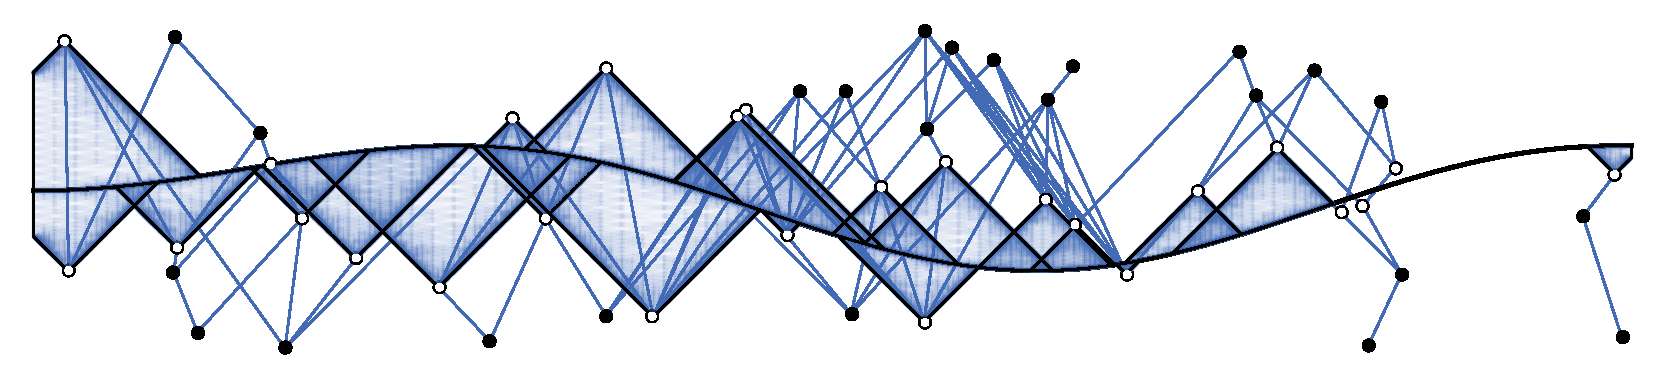
\includegraphics[width=\textwidth]{minmaxplot}
     \caption{Minimal and maximal points about a surface in 2D Minkowski space. The shaded regions illustrate the regions that one must calculate the volume of.}
     \label{fig:Nmin_Nmax}
\end{figure}

If we pick a point $x_0=(0,\mathbf{x})\in \Sigma$ on the surface that has the same spatial coordinates as $x=(t,\mathbf{x})$ then the coordinate time, $t$, is the proper time elapsed along the unique geodesic between $x_0$ and $x$. The volume $V(\Sigma,x)$ then only depends on $t$. Now as $\rho\rightarrow\infty$, we may pick any $\epsilon>0$ such that the contribution to \eqref{eq:nmax} and \eqref{eq:nmin} from points with $|t|>\epsilon$ will be negligible. We assume now that for large enough $\rho$, the region $\left\{|t|<\epsilon\right\}$ is entirely contained in the neighbourhood $U_\Sigma$ in which the GNC are valid.
Equations \eqref{eq:nmax} and \eqref{eq:nmin} can then be simplified as any time, $t$, which is far away from the surface will give rise to a large volume, which will then be exponentially suppressed as $\rho \rightarrow \infty$. More technically, if we choose some finite coordinate distance $\varepsilon$ away from the surface, either to the past or future, then any volume $V(p,\Sigma)$ or $V(\Sigma,q)$ with $|t|>\varepsilon$ will contribute nothing to the integral as $\rho \rightarrow \infty$. This $\varepsilon$ can be chosen arbitrarily close to $0$ allowing one to expand metric in $t$ about $t=0$. This gives

\begin{align}\label{eq:nmax_and_eq:nmin}
\left\langle N_{max}\right\rangle & =\int_{\Sigma}d^{d-1}x\int_{-\varepsilon}^{0}dt\:
h^{\frac{1}{2}}\left(1+
\frac{1}{2}\frac{\dot{h}}{h}t+O(t^2)\right)
 \rho\ e^{-\rho V(-t,\mathbf{x};0,\mathbf{x})}
\\
\left\langle N_{min}\right\rangle & =\int_{\Sigma}d^{d-1}x\int_{0}^{\varepsilon}dt\:
h^{\frac{1}{2}}\left(1+
\frac{1}{2}\frac{\dot{h}}{h}t+O(t^2)\right) \rho\ e^{-\rho V(0,\mathbf{x};t,\mathbf{x})}
\end{align}
where $h\equiv det\left(h_{ij}(0,\mathbf{x})\right)$ and $\dot{}\equiv \frac{\partial}{\partial t}$. The metric determinant has been in expanded in small $t$. The volume functions have been rewritten as follows: $V(x,\Sigma)=V(x,x_0)=V(-t,\mathbf{x};0,\mathbf{x})$ and $V(\Sigma,q)=V(x_0,x)=V(0,\mathbf{x};t,\mathbf{x})$

The only curvy cones that will contribute will have small volumes, as we are restricting ourselves close to the surface. This means that the volumes can be approximated by the volumes of less curvy cones, and it can be shown that higher order corrections, in the approximation scheme, vanish in the limit of $\rho \rightarrow \infty$. This will all be made more precise below. The approximation procedure will be outlined below for a cone to the future of $\Sigma$, as the process for the past cone is nearly identical. Riemann normal coordinates are integral to the following calculation so it is worth noting the relevant formulas before jumping in. 

\section{Riemann Normal Coordinates}

One can always find Riemann normal coordinates (RNC), about a point $p$, by changing from coordinates $x^{\alpha}$ to coordinates $y^{\overline{\alpha}}$ such that in these new coordinates the metric and the Christoffel symbols at $p$ are that of flat space. These conditions  can be expressed as follows

\be\label{eq:RNCMetricTransAtPAndChris}
g_{\overline{\alpha} \overline{\beta}}(p)=\eta_{\overline{\alpha} \overline{\beta}}=A^{\alpha}_{\;\overline{\alpha}}A^{\beta}_{\;\overline{\beta}}g_{\alpha\beta}(p)\;,\;\;\;\;\Gamma^{\overline{\alpha}}_{\;\overline{\beta}\overline{\gamma}}(p)=0
\ee
The $A^{\alpha}_{\;\overline{\alpha}}$ govern the coordinate transformation to linear order, but $O(x^2)$ corrections may be required. To second order the coordinate transformation is given by

\be\label{eq:RNCtotaltrans}
y^{\overline{\alpha}}=A^{\overline{\alpha}}_{\;\beta}x^\beta+\frac{1}{2}A^{\overline{\alpha}}_{\;\alpha}\Gamma^{\alpha}_{\;\beta\gamma}(p)x^\beta x^\gamma+O(x^3)
\ee
and the inverse transformation is just

\be\label{eq:RNCinversetrans}
x^{\alpha}=A^{\alpha}_{\;\overline{\beta}}y^{\overline{\beta}}+O(y^2)
\ee
One finds that the $A^{\alpha}_{\;\overline{\alpha}}$ also satisfy

\be\label{eq:RNCeqnforA}
A^{\overline{\alpha}}_{\;\mu}A^{\mu}_{\;\overline{\beta}}=\delta^{\overline{\alpha}}_{\;\overline{\beta}}\;,\;\;\;\;A^{\alpha}_{\;\overline{\mu}}A^{\overline{\mu}}_{\;\beta}=\delta^{\alpha}_{\;\beta}
\ee
These relations for RNC will cover all that will be needed in this discussion.

\section{Lightcone Volumes}

The volumes of the truncated lightcones can be found as follows. Consider the past lightcone emanating at the point $p_0=(T,\mathbf x_0)$. There is a unique point $q_0=(0,\mathbf x_0)$ on $\Sigma$ associated with $p_0$, separated from $p_0$ by a proper time $T$. 

The volume of this cone is given by

\be\label{eq:VolumeWithNoSimplifications}
V(0,\mathbf{x}_0;T,\mathbf{x}_0)=\int_{\mathcal{X}} d^d x\;\sqrt{-g}
\ee
where the integration region, $\mathcal{X}:= J^-(p_0)\bigcap J^+(\Sigma)$ will be some complicated thing. As we are dealing with points close to the surface we can use the  Riemann normal coordinates $y^{\overline{\mu}}$, defined as above, about the point $q_0$ (the point $q_0$ being the origin of our RNC system). One finds that $A^0_{\;\overline{0}}=1$, $A^0_{\;i}=0$ and $\delta_{\overline{i}\overline{j}}=A^i_{\;\overline{i}}A^j_{\;\overline{j}}h_{ij}(0,\mathbf{x}_0)$. It can be shown that the volume integral reduces to \cite{Khetrapal_Sumati:Causal_Diamond_Volume}

\be\label{eq:VolumeWithRNC}
V(0,\mathbf{x}_0;T,\mathbf{x}_0) =\int_{\mathcal{X}}d^dy+\int_{\mathcal{X}_0}d^dy\left(-\frac{1}{6}R_{\overline{\mu}\overline{\nu}}(q_0)y^{\overline{\mu}}y^{\overline{\nu}} \right)+O(T^{d+3})
\ee
where $\mathcal{X}_0=\left\lbrace y^{\overline{\mu}} \mid 0\leq y^{\overline{0}}=\overline{t}\leq T\; ,\; \sqrt{(y^{\overline{1}})^2+(y^{\overline{2}})^2+...+(y^{\overline{d-1}})^2}\leq T-\overline{t} \right\rbrace$ is what we call the \textit{flat cone}, and $R_{\overline{\mu}\overline{\nu}}(q_0)$ is the Ricci tensor in RNC evaluated at $q_0$. The arguments of the volume function need not be changed as the volume only depends on the points in the manifold, $q_0$ and $p_0$. The \textit{flat cone} term comes in at $O(T^{d+2})$ so the volume we have to calculate has reduced to

\be\label{eq:VolumeToLowestOrder}
V(0,\mathbf{x}_0;T,\mathbf{x}_0) =\int_{\mathcal{X}}d^dy+O(T^{d+2})
\ee
Terms of $O(T^{d+2})$ can be retained till the end, but in the limit, $\rho\rightarrow\infty$, they vanish. This will be proved below.

The boundaries of $\mathcal{X}$ must now be figured out in order to do this integral. First we look at the top part of the cone. From \cite{Khetrapal_Sumati:Causal_Diamond_Volume} it can be shown that the first curvature correction to the top part of the cone comes in at $O(T^{d+2})$ and so can be ignored for our purposes. This means that the top can be treated as a that of a \textit{flat cone} and so points on the boundary obey the equation $\sqrt{(y^{\overline{1}})^2+(y^{\overline{2}})^2+...+(y^{\overline{d-1}})} = T-\overline{t}$.

The bottom surface of the cone was defined in terms of GNC to be $t=0$, so we can use (\ref{eq:RNCtotaltrans}) to find the equation for the surface in RNC. Equation (\ref{eq:RNCtotaltrans}) gives

\be\label{eq:BottomSurfaceWithGNC}
y^{\overline{0}}=\overline{t}=\frac{1}{2}\Gamma^{0}_{\;ij}(0,\mathbf{x}_0)x^i x^j+O(x^3)
\ee
The first part on the right vanishes as $A^{\overline{0}}_{\;\mu}x^{\mu}=x^0$ (as $A^{\overline{0}}_{\;i}=0$ and $A^{\overline{0}}_{\;0}=1$) and $x^0=t=0$ for the bottom surface. Using the inverse RNC relation (\ref{eq:RNCinversetrans}) one can find the equation for the bottom surface entirely in RNC.

\be\label{eq:BottomSurface}
\overline{t}=\frac{1}{2}\Gamma^{0}_{\;ij}(0,\mathbf{x}_0)A^{i}_{\;\overline{i}}A^{j}_{\;\overline{j}}y^{\overline{i}} y^{\overline{j}}+O(y^3)
\ee

This equation can be written in terms of the radial coordinate of the cone, $r=\sqrt{(y^{\overline{1}})^2+...+(y^{\overline{d-1}})^2}$, as

\be\label{eq:RadialBottomSurface}
\overline{t}=\frac{1}{2}\left(\Gamma^{0}_{\;ij}(0,\mathbf{x}_0)A^{i}_{\;\overline{i}}A^{j}_{\;\overline{j}}\frac{y^{\overline{i}} y^{\overline{j}}}{r^2}\right)r^2+O(y^3)=\frac{1}{2}f(\mathbf{x}_0,\phi)r^2+O(y^3)
\ee
where $\phi$ stands for all the angular coordinates $\phi_1,..,\phi_{d-2}$. The function $f(\mathbf{x}_0,\phi)$ depends on $\mathbf{x}_0$ as $\Gamma^{0}_{\;ij}$ and $A^{i}_{\;\overline{i}}$ will, in general, be different for a different point on the surface. One can see that $f(\mathbf{x}_0,\phi)$ depends on the angles, $\phi$, by substituting the relations below into (\ref{eq:RadialBottomSurface})

\begin{align}\label{eq:SphericalCoords}
y^{\overline{1}} &= r \cos(\phi_1) \nonumber \\
y^{\overline{2}} &= r \sin(\phi_1) \cos(\phi_2) \nonumber \\
y^{\overline{2}} &= r \sin(\phi_1) \sin(\phi_2) \cos(\phi_3) \nonumber \\
    &\vdots \nonumber \\
y^{\overline{d-2}} &= r \sin(\phi_1) \cdots \sin(\phi_{d-3}) \cos(\phi_{d-2}) \nonumber \\
y^{\overline{d-1}} &= r \sin(\phi_1) \cdots \sin(\phi_{d-3}) \sin(\phi_{d-2})
\end{align}

With the boundaries of the integration region in place, we can now write down the integral explicitly, in spherical coordinates:

\be\label{eq:VolumeIntegralSpherical}
V(0,\mathbf{x}_0;T,\mathbf{x}_0)=\int_{S^{d-2}}
d\Omega_{d-2}
\int_{0}^{r_{max}(\phi)}r^{d-2}dr
\int_{\frac{1}{2}f(\mathbf{x}_0,\phi)r^2}^{-r+T}
d\overline{t}+O(T^{d+2})
\ee
where $r_{max}(\phi)$ is the radial coordinate of where the bottom surface meets the top part of the cone at an angle $\phi$, shown in \ref{fig:cone_plot}. To find this one needs to solve $\frac{1}{2}f(\mathbf{x}_0,\phi){r_{max}}^2(\phi)=-r_{max}(\phi)+T$ and take the positive solution. The solution can be expanded in $T$ and is simply $r_{max}=T+O(T^2)$, with angular dependent terms contributing at $O(T^2)$. The $O(T^2)$ term will contribute at $O(T^{d+2})$ in the integral and so can be ignored. Substituting $r_{max}=T$ into (\ref{eq:VolumeIntegralSpherical}) means it can be evaluated to give

\begin{figure}
  \centering
    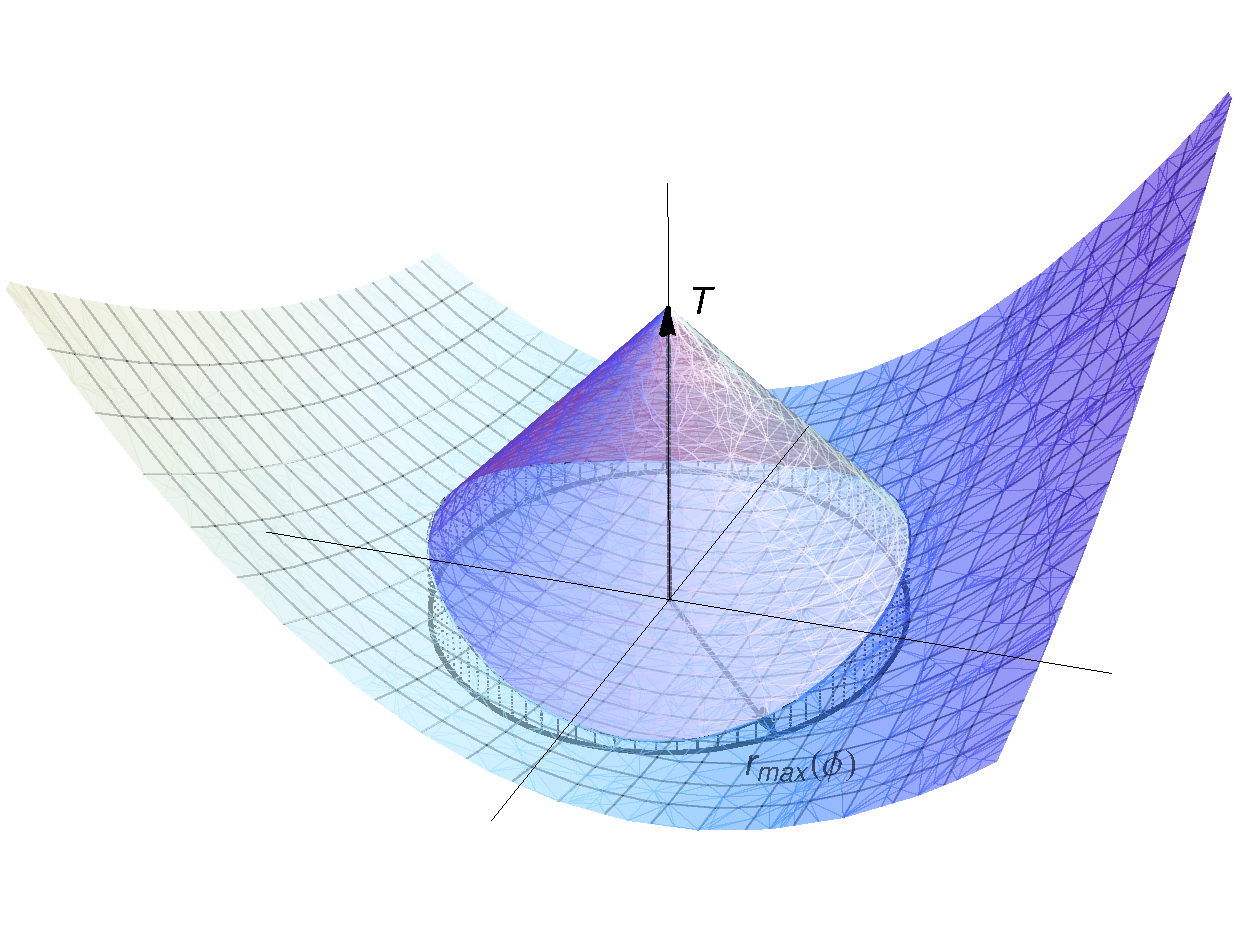
\includegraphics[scale=0.6]{coneplot}
     \caption{The size of the region inside the top and bottom bounding surfaces is the volume we want to calculate.}
     \label{fig:cone_plot}
\end{figure}

\be\label{eq:VolumeNoK}
V(0,\mathbf{x}_0;T,\mathbf{x}_0)
=\frac{A_{d-2}}{d(d-1)}T^d\left(1-\frac{d}{2(d+1)}\Gamma^{0}_{\;ij}(0,\mathbf{x}_0)A^{i}_{\;\overline{i}}A^{j}_{\;\overline{j}}\delta^{\overline{i}\overline{j}}T\right)
+O(T^{d+2})
\ee
where $A_{d-2}$ is the $d$-$2$ dimensional volume of a $d$-$2$ dimensional sphere and the $\delta^{\overline{i}\overline{j}}$ has come from the fact that cross terms ($\overline{i}\neq \overline{j}$) vanish under the angular integration. The defining relations for $A^{i}_{\;\overline{i}}$ can be rearranged to give $A^{i}_{\;\overline{i}}A^{j}_{\;\overline{j}}\delta^{\overline{i}\overline{j}}=h^{ij}(0,\mathbf{x}_0)$. In GNC it can be shown that the extrinsic curvature is given by

\be\label{eq:K}
K(0,\mathbf{x}_0)
=g^{\mu\nu }\nabla_{\mu}n_{\nu}
=-\Gamma^{0}_{\;ij}(0,\mathbf{x}_0)h^{ij}(0,\mathbf{x}_0)=-\frac{1}{2}\frac{\dot{h}(0,\mathbf{x}_0)}{h(0,\mathbf{x}_0)}
\ee
which means that the first correction to the volume of the cone depends on $K(0,\mathbf{x}_0)$, and thus the approximate volume of the cone is

\begin{align}
V(0,\mathbf{x}_0;T,\mathbf{x}_0)
&=\frac{A_{d-2}}{d(d-1)}T^d\left(1+\frac{d}{2(d+1)}K(0,\mathbf{x}_0)T\right)
+O(T^{d+2}) \label{eq:TopVolumeWithK}\\
V(-T,\mathbf{x}_0;0,\mathbf{x}_0)
&=\frac{A_{d-2}}{d(d-1)}T^d\left(1-\frac{d}{2(d+1)}K(0,\mathbf{x}_0)T\right)
+O(T^{d+2}) \label{eq:BottomVolumeWithK}
\end{align}
where (\ref{eq:BottomVolumeWithK}) is the volume of the cone with its tip below the surface, and can be found from similar arguments.

\section{Final Stretch of the Proof}

Let us now use these volume functions in the expressions for $\left\langle N_{max}\right\rangle$ and $\left\langle N_{min}\right\rangle$ to calculate the $\left\langle N_{max}-N_{min}\right\rangle$ term in equation (\ref{GH_boundary_to_causet}) as $\rho \rightarrow \infty$. We have

\begin{gather}\label{eq:NmaxNminStart}
\begin{aligned}
\lim_{\rho \to \infty}\left\langle N_{max}-N_{min} \right\rangle &= \\
\lim_{\rho \to \infty}\rho
\int_{\Sigma}d^{d-1}x & \int_{-\varepsilon}^{0}dt\
h^{\frac{1}{2}}\left(1+
\frac{1}{2}\frac{\dot{h}}{h}t-\rho B(-1)^{d}t^{d+1}+\rho O(t^{d+2})\right)e^{-\rho A(-1)^{d}t^{d}} \\
-\rho\int_{\Sigma}d^{d-1}x &
\int_{0}^{\varepsilon}dt\
h^{\frac{1}{2}}\left(1+
\frac{1}{2}\frac{\dot{h}}{h}t-\rho Bt^{d+1}+\rho O(t^{d+2})\right)e^{-\rho At^{d}}
\end{aligned}
\end{gather}
where we have defined

\begin{gather}\label{A_and_B_defn}
\begin{aligned}
A & \equiv \frac{A_{d-2}}{d(d-1)} \\
B & \equiv \frac{A_{d-2}}{2(d-1)(d+1)}K(0,\mathbf{x})
\end{aligned}
\end{gather}
and we have Taylor expanded the $O(t^{d+1})$ parts of the volume functions, in small $t$, from the exponents. If we change to $u=-t$ in the first part on the right hand side, and $u=t$ on the second part then the integral can be simplified to

\be\label{eq:NmaxNminSimplified}
\lim_{\rho \to \infty}\left\langle N_{max}-N_{min} \right\rangle=
\lim_{\rho \to \infty}\rho
\int_{\Sigma}d^{d-1}x \int_{0}^{\varepsilon}du\
h^{\frac{1}{2}}\left(-\frac{\dot{h}}{h}u+2\rho B u^{d+1}+\rho Cu^{d+2}+\rho O(u^{d+3}) \right)e^{-\rho Au^{d}}
\ee
where $C$ is the coefficient of $O(u^{d+2})$ terms. This term has been included as showing that it, and higher powers, vanish as $\rho \rightarrow\infty$ will prove our claim that no higher order terms are needed. To prove this we need to show that the following integral vanishes

\be\label{eq:VanishingOrderIntegral}
\lim_{\rho \to \infty}\rho^{\frac{2}{d}-1}\rho\int_{0}^{\varepsilon}du\
\rho u^{d+n}e^{-\rho Au^{d}}=\lim_{\rho \to \infty}\rho^{\frac{2}{d}+1}\int_{0}^{\varepsilon}du\
u^{d+n}e^{-\rho Au^{d}}
\ee
where $n\in\mathbb{N}$. We have left the powers of $\rho$ separated on the left side to show where they have come from. The first $\rho^{\frac{2}{d}-1}$ comes from (\ref{GH_boundary_to_causet}) and is needed to balance dimensions. This must be included in order to take the limit properly. We then make the substitution $z=\rho Au^{d}$ to transform the integral into that of an incomplete gamma function, which in the limit becomes a complete gamma function

\be\label{eq:GammaVanishingOrderIntegral}
\lim_{\rho \to \infty}\rho^{\frac{1-n}{d}}\frac{A^{\frac{n+1}{d}+1}}{d}\int_{0}^{\rho A\varepsilon^d}dz\
z^{\frac{n+1}{d}}e^{-z}\sim\lim_{\rho \to \infty}\rho^{\frac{1-n}{d}}\int_{0}^{\infty}dz\
z^{\left[\left(\frac{n+1}{d}+1\right)-1 \right]}e^{-z}\sim\lim_{\rho \to \infty}\rho^{\frac{1-n}{d}}\Gamma\left(\frac{n+1}{d}\right)
\ee
The $\rho$ in the limit of the second expression has been taken to $\infty$. The power of $z$ in this integral has been written in this manner so it can be more easily recognised as being of gamma function form, $\Gamma(t)=\int_{0}^{\infty}z^{t-1}e^{-z}dz$. One can see from above that if $n>1$ then this term will vanish, thus proving that terms of $O(u^{d+2})$ or higher will go to $0$ in the limit $\rho\rightarrow\infty$.

We use this fact and the method of putting the integrals into a gamma function form to evaluate (\ref{eq:NmaxNminSimplified}). One also sees that we have terms like $\frac{\dot{h}}{h}$, and from (\ref{eq:K}) we know that these can be written in terms of the extrinsic curvature, $K(0,\mathbf{x})$. We find then that (\ref{eq:NmaxNminSimplified}) reduces to

\be\label{eq:nmax_eq:nmin_end}
\lim_{\rho \to \infty}\left\langle N_{max}-N_{min} \right\rangle=\lim_{\rho \to \infty}
\rho^{1-\frac{2}{d}}\frac{2(d+2)}{d(d+1)}
\left[\frac{A_{d-2}}{d(d-1)}\right]^{-\frac{2}{d}}
\Gamma\left(\frac{2}{d}\right)\int_{\Sigma}d^{d-1}x\
\sqrt{h}K(0,\mathbf{x})
\ee
$K(0,\mathbf{x})$ is evaluated at the surface and is therefore the same $K$ as in equation (\ref{GH_boundary_to_causet}). We can therefore conclude that to make (\ref{GH_boundary_to_causet}) true we need a factor $\rho^{\frac{2}{d}-1}$ to cancel the factors of $\rho$ above, and a value of $c_d$ equal to that of equation (\ref{Cn}). The factor of $\rho$ needed is exactly that required on dimensional grounds, thus we have proved that (\ref{GH_boundary_to_causet}) is in fact true in general.


\end{document}